\mysection{エミッタ接地回路のバイアス電圧$v_{be}$の設定(原理・計算)}
エミッタ接地増幅回路の基本原理を図\ref{emitter_genri}に示す。
\begin{figure}[htb]
  \begin{center}
  \subfigure[エミッタ接地回路の原理図]{	% 副題なし
  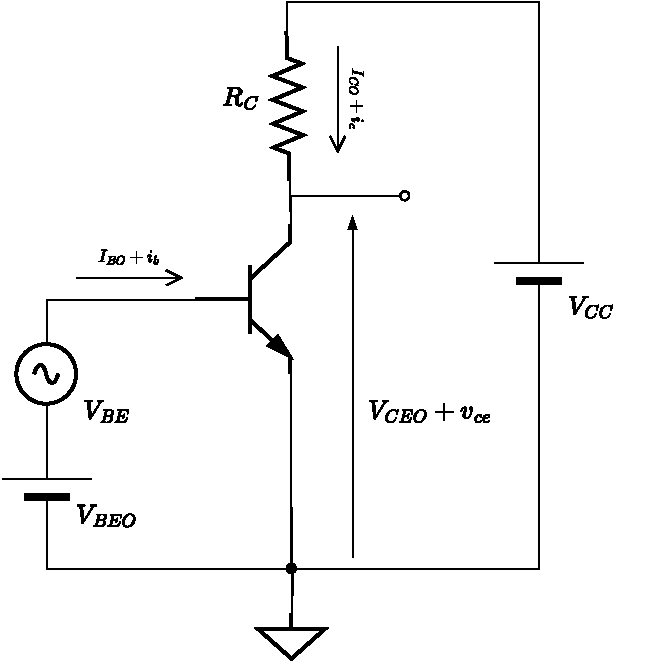
\includegraphics[width=.33\columnwidth]{img/37.pdf}
  }
  \subfigure[$V_{BE}$-$I_E$特性]{
  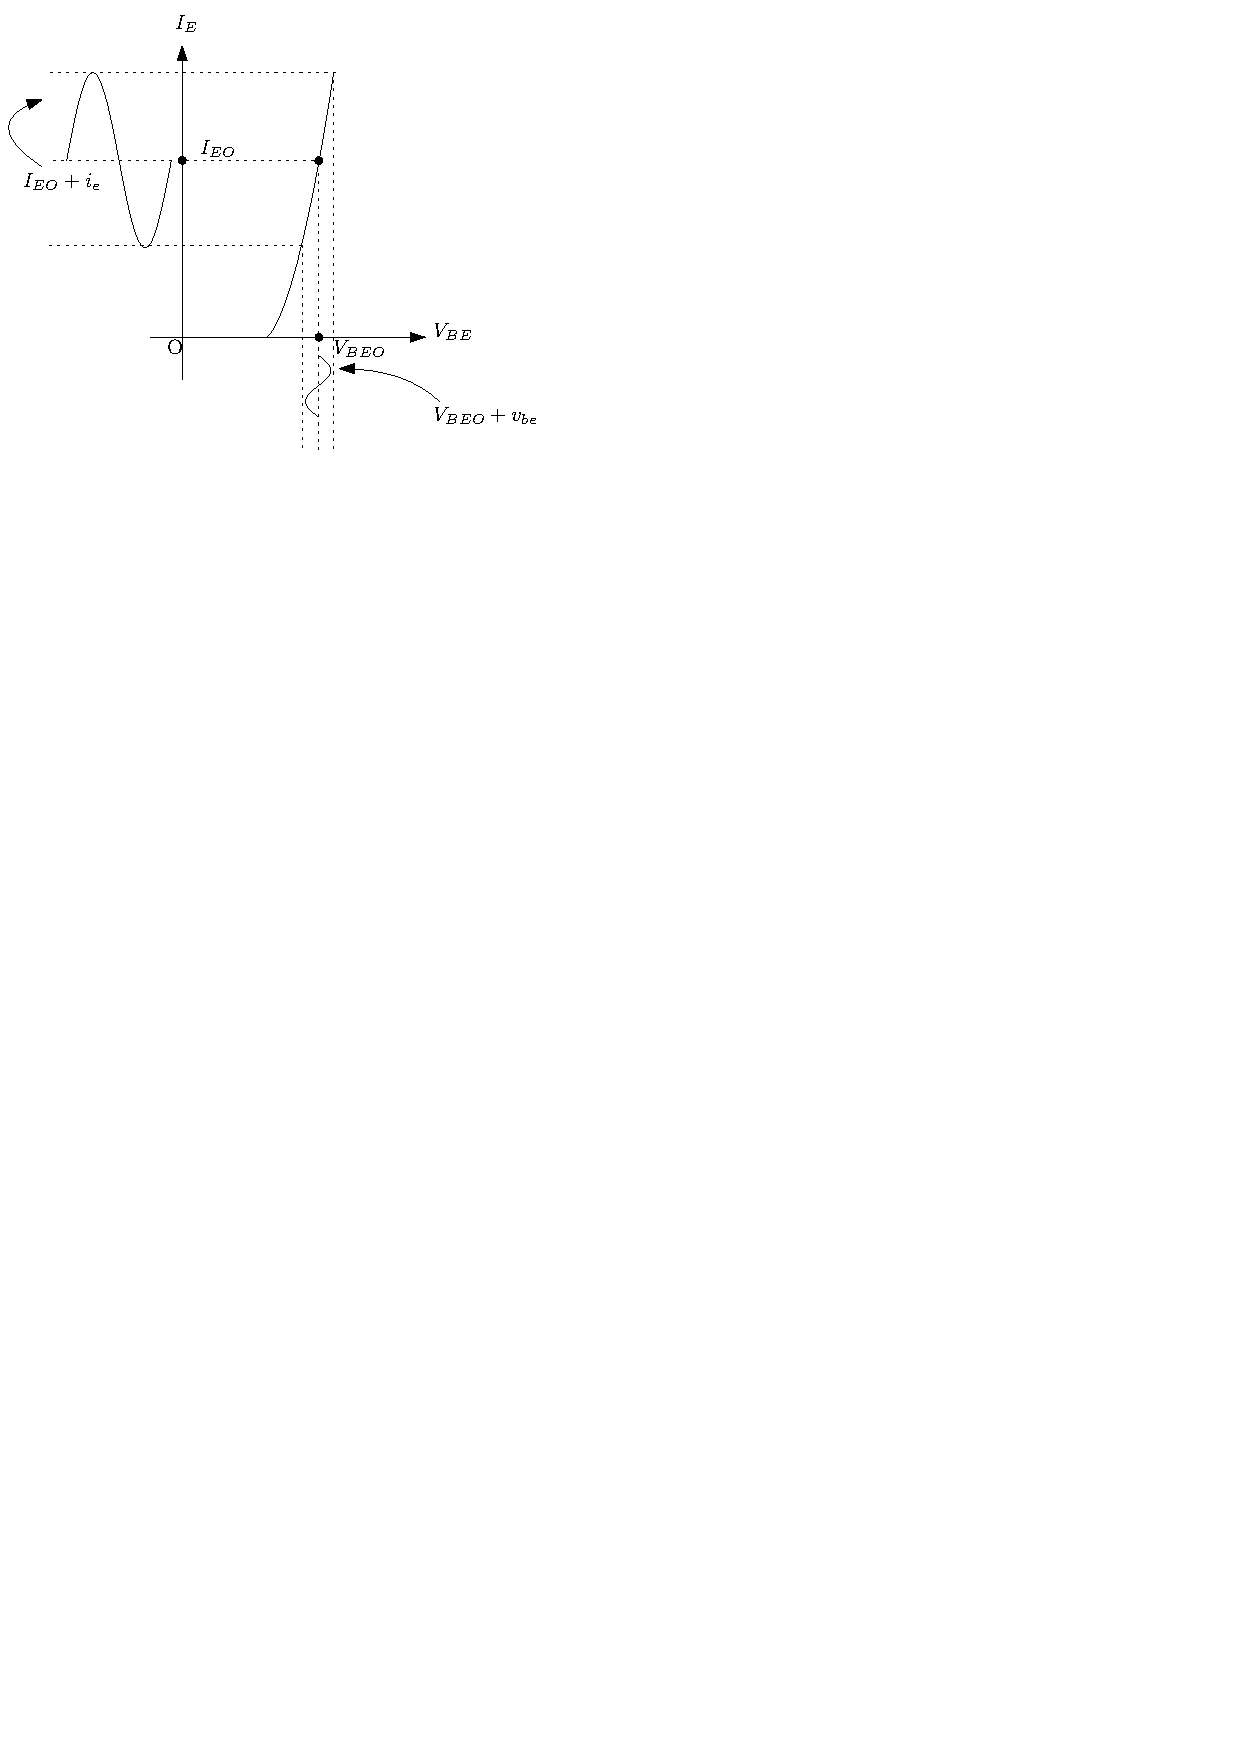
\includegraphics[width=.33\columnwidth]{img/38.pdf}
  }
  \subfigure[$I_C$-$V_{CE}$特性]{
  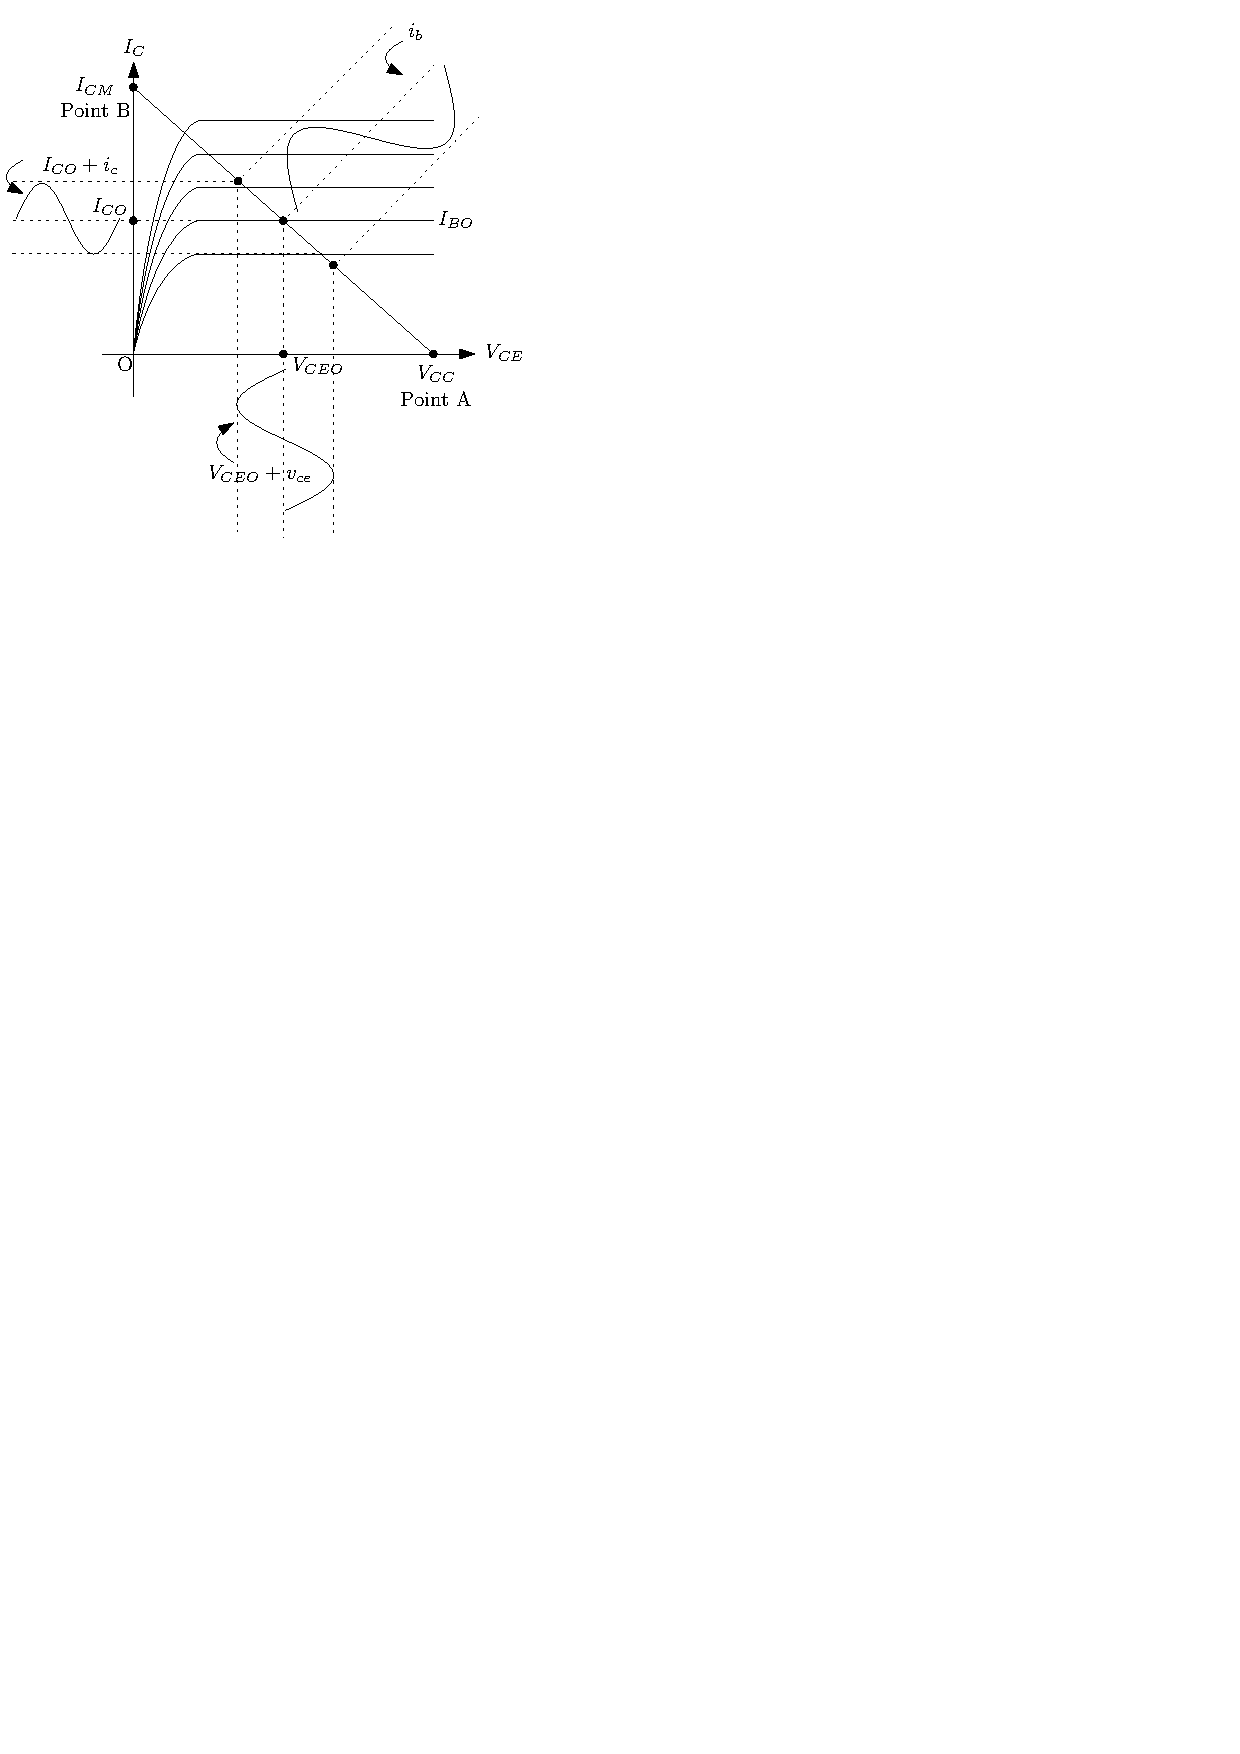
\includegraphics[width=.33\columnwidth]{img/39.pdf}
  }
  \caption{エミッタ接地回路の基本原理}
  \label{emitter_genri}
  \end{center}
\end{figure}

\begin{enumerate}
  \setlength{\parskip}{0cm} % 段落間
  \setlength{\itemsep}{0cm} % 項目間
  \item バイアス電圧 $V_{BEO}$ を印加
  \item 交流電圧 $v_{be}$ を加えると、ベース電流は、動作点 $I_{BO}$ を中心に $i_b$ 変化する
  \item コレクタ電流は動作点 $I_{CO}$ を中心に $i_c$ 変化する。
  \item コレクタ-エミッタ間電圧は、動作点 $V_{CEO}$ を中心に $v_{ce}$ 変化する
\end{enumerate}
\mysubsection{バイアス電圧$V_{BE}$の設計手順}
\begin{enumerate}
  \setlength{\parskip}{0cm} % 段落間
  \setlength{\itemsep}{0cm} % 項目間
  \item $I_C$-$V_{CE}$ 特性に負荷線を引く (\textbf{$R_C$ を決める})\\
  $V_{CC}$、$I_{CM}$ は自分で決める。\\
  $V_{CC} = 10$ V $I_{CM} = 11$ mA として計算\\
  $V_{CE} = 0$ の時、($v_{ce}$ を短絡)$I_{CM} = \frac{V_{CC}}{R_C}$\\
  -$I_C = 0$ の時、($R_C$ で電圧降下が起きない。$R_C$ を短絡) $V_{CEM} = V_{CC}$\\
  $V_{CC} = \frac{10}{R_C}  より、$
  \begin{align}
    \frac{V_{CC}}{R_C} = I_{CM} = \frac{10}{R_C} = 11 \textrm{mA}
  \end{align}
  よって、
  \begin{align}
    R_C = 909.0909 \Omega
  \end{align}
  $(0, \frac{V_{CC}}{R_C})$、$(V_{CC}, 0)$を通る直線は、
  \begin{align}
    I_C = - \frac{1}{R_C} V_{CE} + \frac{V_{CC}}{R_C} = \frac{10 - V_{CE}}{909.09}
  \end{align}

  \item $V_{CE}$ の動作点 $V_{CEO}$ を求める ($v_{ce}$ は自分で決める。±の値になる)\\
  コレクタエミッタ間電圧 $V_{CE}$ の振幅が大きく取れるように動作点を設定する。\\
  エミッタ接地回路では、コレクタエミッタ間電圧 $V_{CE}$ の動作点は電源電圧 $V_{CC}$ と 0 V
  の真ん中付近に $V_{CEO}$ を設定する。
  今回は、$V_{CC} = 10$ Vであるため、$V_{CEO} = \frac{V_{CC}}{2} = 5\textrm{V}$を動作点とする。
  また、今回は$v_{ce} = \pm 0.9$ Vとして計算する。
  \item コレクタ電流 $i_c$ の動作点 $I_{CO}$ を求める。\\
  $I_C-V_{CE}$ 特性で、$V_{CEO}$ を決めたとき、その振れ幅に対応する $i_c$ と、$V_{CEO}$ に対する、$I_{CO}$ (コレクタ電流の動作点)が決まる。($I_{CO}$が決まると、$I_{BO}$が決まる。)
  \begin{align}
    I_{CO} = \frac{V_{CC}}{2R_C} = \frac{V_{CEO}}{R_C} = \frac{5}{909.09} \approx 5.5 \textrm{mA}    
  \end{align}
  $V_{CE} = 5 - 0.9 = 4.1$ Vの場合、$I_C \approx 6.49$ mA\\
  $V_{CE} = 5 +0.9 = 5.9$ Vの場合、$I_C \approx 4.51$ mA\\
  $I_C$の振れ幅は、$6.49 - 4.51 = 1.98$ mAであるため、
  $I_C = I_{CO}+i_c = 5.5 \pm 0.99$ mAと決まる。
  \item ベースエミッタ間電圧 $V_{BE}$ の動作点 $V_{BEO}$ を求める\\
  $I_C \approx I_E$ とし、LTSpiceでシミュレーションした$I_E-V_{BE}$ 特性の値をカーソルで読み取る。\\
  $I_C = 5.5 + 0.99$ mA の場合、$I_E-V_{BE}$ 特性より $V_{BE} = 0.7427$ V\\
  $I_C = 5.5 - 0.99$ mA の場合、$I_E-V_{BE}$ 特性より $V_{BE} = 0.73365$ V\\
  $I_C = I_{CO} = 5.5$ mA の場合、$V_{BEO} = 0.7386$ V
\end{enumerate}